\chapter{Desenvolvimento}
\section{Hardware}
\subsection{TIVA e seus pontos fracos}
\subsection{STM32F769I-DISCO e suas vantagens}
\subsection{Possíveis hosts para o device}
\subsection{Componentes}
\section{Firmware}
\subsection{HAL, BSP e CMSIS}
Este projeto conta com a utilização de camadas de abstração de hardware que ???. Entre elas, estão a HAL (Hardware Abstraction Layer), BSP (Board Support Package) e CMSIS (Common Microcontroller Software Interface Standard).
\\[10pt]
% https://en.wikipedia.org/wiki/Hardware_abstraction
% https://www.techopedia.com/definition/4288/hardware-abstraction-layer-hal
% https://emteria.com/learn/hardware-abstraction-layer


A \textit{Hardware Abstraction Layer (HAL)} é uma camada de bibliotecas de código que possui a função de entregar uma interface de desenvolvimento padronizada que permita interações com o hardware sem necessidade do conhecimento direto do hardware em questão 
% [[FONTE]](https://emteria.com/learn/hardware-abstraction-layer).

Isso permite uma maior portabilidade do código, o qual se torna compatível com qualquer hardware que também esteja incluso nessa camada de abstração.
Uma HAL é comumente acessível como uma API que realiza o trabalho de inicialização, configuração e acesso a um hardware específico. Para este projeto, foi utilizada a HAL V1.2.6, lançada em 29 de junho de 2018.
\\[10pt]

A \textit{Board Support Package (BSP)} é uma coleção de APIs, drivers e arquivos de configuração que tem como intuito facilitar o desenvolvimento em uma placa específica. 
Para este projeto, foi utilizado a BSP da placa STM32F769I-DISCO.
\\[10pt]

O \textit{Common Microcontroller Software Interface Standard (CMSIS)} é um conjunto de ferramentas, \textit{frameworks} e funcionalidades que implementam funcionalidades, mecânicas e utilidades comumente utilizadas no desenvolvimento embarcado, com o intuito de reduzir o atrito inicial do desenvolvimento, evitar re-trabalhos e reduzir e o tempo até o mercado de um produto até o mercado. Ele funciona em paralelo à Hardware Abstraction Layer, inclusive dependendo da versão específica dessa abstração para alguma de suas funcionalidades.

% [https://www.arm.com/technologies/cmsis#:~:text=Common Microcontroller Software Interface Standard,to market for new devices](https://www.arm.com/technologies/cmsis#:~:text=Common%20Microcontroller%20Software%20Interface%20Standard,to%20market%20for%20new%20devices).

% https://deepbluembedded.com/stm32-hal-library-tutorial-examples/

% https://www.st.com/resource/en/product_training/STM32G0-Ecosystem-STM32Cube-G0-Firmware-Package.pdf

% https://arm-software.github.io/CMSIS_5/General/html/index.html

\subsection{Configuração como dispositivo de áudio USB}
Algumas configurações precisam ser enviadas na conexão com a fonte para que o dispositivo seja reconhecido corretamente como um dispositivo de áudio. Duas das principais configurações necessárias são os VIDs e PIDs, ambos números de 16 bits tipicamente representados em hexadecimal.

% https://en.wikipedia.org/wiki/USB_Implementers_Forum

\textit{VIDs (Vendor IDs)} são números que identificam um fabricante ou fornecedor de dispositivos USB. Esse identificador é fornecido pelo USB Implementers Forum, necessitando de licenças anuais de custo elevado. Algumas fabricantes de microcontroladores permitem o uso de sua licença para fins não comerciais ou de pequena escala. Este projeto utiliza o vendor ID da STMicroelectronics (0x0483)

\textit{PIDs (Product IDs)} são números que identificam o dispositivo de maneira diferente para o sistema operacional ao qual ele está se conectando. Esse identificador varia de acordo com cada fornecedor.

Para esse dispositivo ser reconhecido como uma saída de áudio da STMicroelectronics, ele precisa informar ao sistema operacional que está se conectando o identificador 0x5730.

\subsection{Armazenamento (buffer circular)}
Como o modo de tranferência não possui correção de erro nem bufferização de dados, precisamos utilizar de um armazenamento temporário para podermos manipular e enviar o dado para frente.
\begin{figure}[!h]
  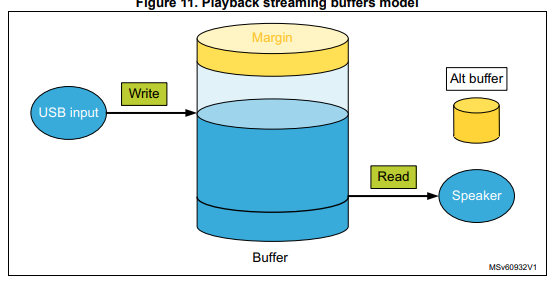
\includegraphics[scale=0.5]{figuras/circular-buffer.png}
  \caption{!! TROCAR POR VERSÃO DE AUTORIA PRÓPRIA !!}
  \label{fig:circularBuffer}
\end{figure}

Para se adequar ao padrão produtor-consumidor utilizado na transmissão USB, um buffer circular é utilizado. 

Ponteiros de leitura e escrita são utilizados para indicação de onde novos pacotes devem ser lidos e onde devem ser escritos, respectivamente. O ponteiro de leitura é administrado pelo nó de saída de áudio, e o de escrita pelo nó de entrada USB.

!!Explicar como dados são inseridos no buffer!!. O ponteiro de escrita é então incrementado para refletir a presença dos novos dados presentes no buffer.

!! Explicar como dados são consumidos do buffer!!. O ponteiro de leitura é incrementado para refletir esta leitura.

Através de DMA, os dados são então transferidos para o SAI (e em sequência para o codec).

Para todas as escritas e leituras serem de uma área contínua de memória, uma margem é adicionada ao *buffer*. Isso permite que dados sejam escritos de maneira contínua, mesmo caso o ponteiro de escrita esteja próximo do fim do buffer.

Caso dados sejam escritos de forma que ultrapassem o fim do buffer, a quantidade restante é escrita na margem. Posteriormente, esses dados são corretamente re-escritos no começo do buffer. 

Em casos que não existem dados suficientes para serem escritos ao SAI, um buffer alternativo contendo apenas zeros é utilizado.


\subsection{Processamento de sinal (interceptador)}
Para possibilitar a alteração dos dados recebidos antes que eles sejam transmitidos ao nó de saída, um interceptador foi criado e adicionado como passo intermediário.

O interceptador é um conjunto de métodos que tem como objetivo receber o posicionamento dos dados originais no \textit{buffer}, e transformá-los de acordo com o filtro especificado. Essa transformação é feita antes que o ponteiro de leitura atinja essa parte do \textit{buffer}.

São enviadas informações de posição inicial dos dados, tamanho do pacote, e ponteiros de função para os filtros que devem ser aplicados a cada canal (direito e esquerdo)

Os dados são então iterados em \textit{frames} que possuem informação de dois samples (referentes aos dois canais stereo).

Cada um dos samples dos canais são então armazenados em variáveis temporárias. 

Cada filtro provido é então aplicado ao sample específico a seu canal, modificando-o. 

Finalmente, os samples são convertidos novamente em um único frame, e o valor final desse frame é atribuído à posição original do frame provido no \textit{buffer}.

\subsection{IHM (LCD + Touch)}
A interface homem-máquina é feita com a utilização do LCD embarcado na placa de desenvolvimento. Através dela, o usuário pode verificar a situação atual do sistema, incluindo quais filtros estão ativos no momento.

!! SCREENSHOT 1 !!

O dispositivo também conta com resposta à toque, permitindo com que o usuário interaja diretamente com os dados mostrados em tela. Um sistema de botões radiais foi desenvolvido para permitir que o usuário possa alternar entre os filtros em tempo real.

\section{PDS}
